\chapter{Prezentacja aplikacji}
Aplikacja po uruchomieniu wyświetla domyślną stronę (Home), na której wyświetlają się informację. Pierwszą rzeczą jaką należy zrobić po uruchomieniu jest zalogowanie się lub rejestracja.
\begin{figure}[H]
	\centering
	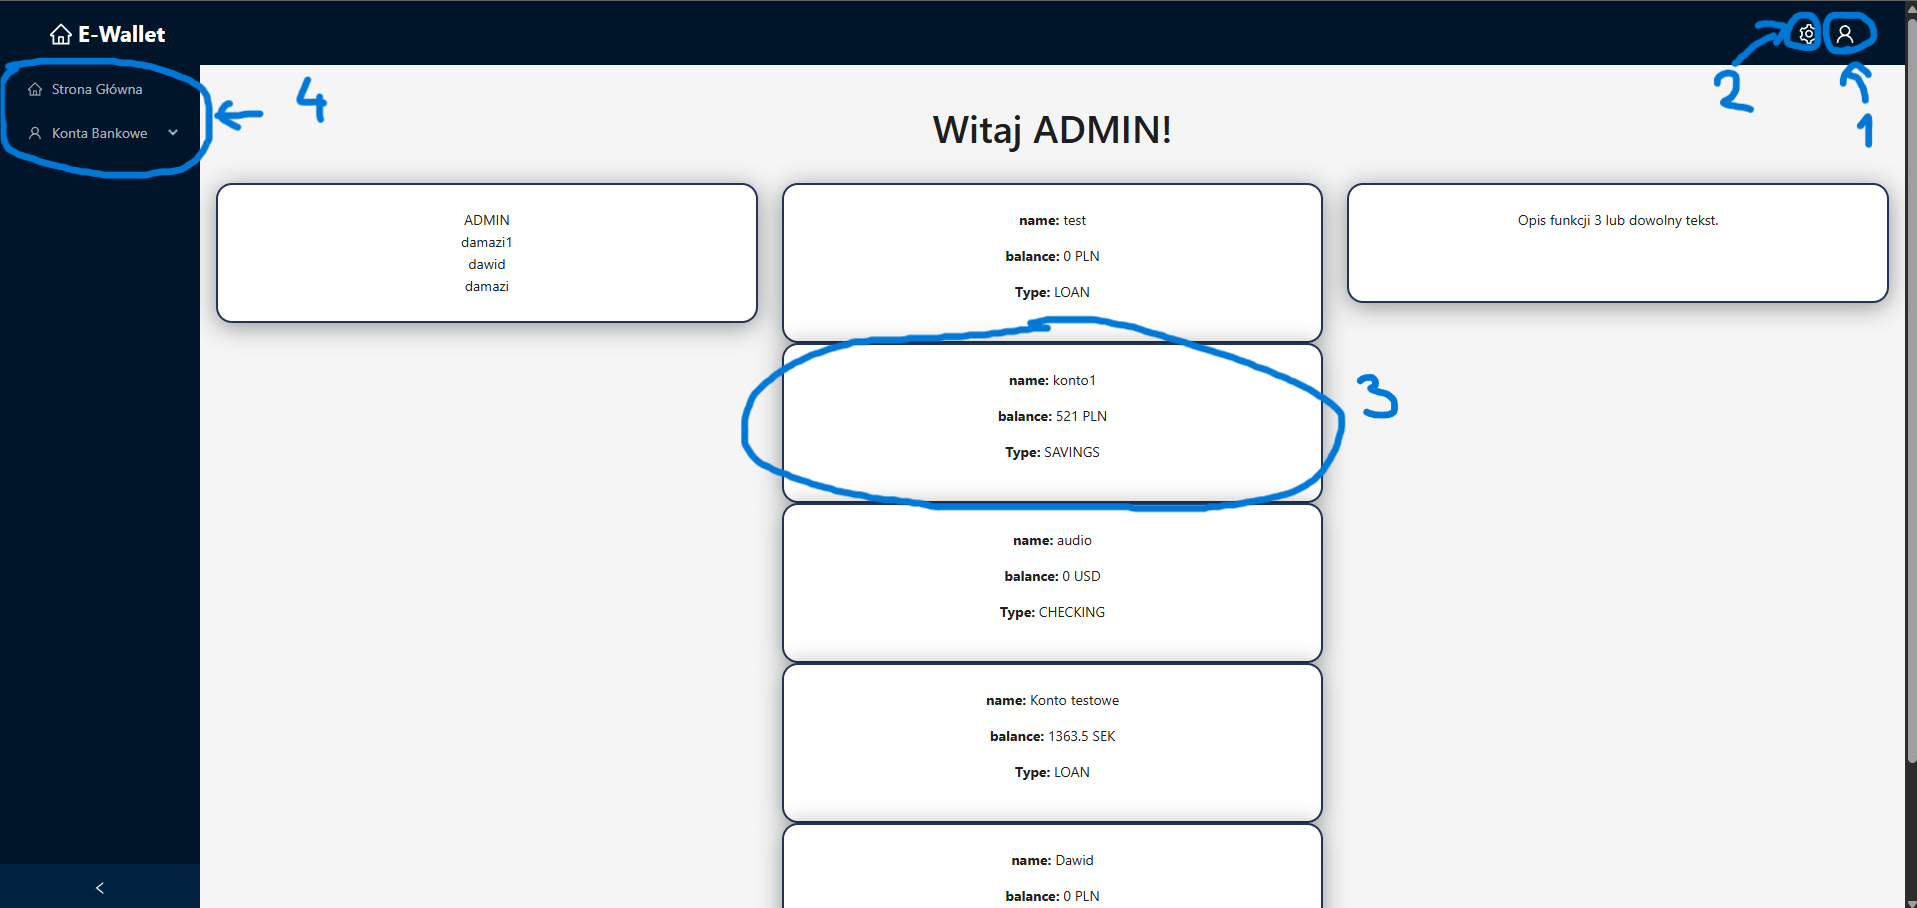
\includegraphics[width=0.7\linewidth]{images/HomePage}
	\caption{Strona startowa po zalogowaniu}
	\label{fig:homepage}
\end{figure}
\begin{itemize}
	\item Pierwszy zaznaczony element na stronie to aktualnie zalogowany użytkownik, po kliknięciu w ikonę użytkownika wyświetli się informacja o profilu oraz możliwość wylogowania w liście wysuwanej (Dropdown Menu).
	\item Drugim elementem są ustawienia. Możemy tu ustawić motyw strony.
	\item Trzeci element to kafelki znajdujące się po środku (Card). Po kliknięciu w nie zostaniemy przeniesieni do odpowiedniego konta.
	\item Czwarty element to lista wysuwana z boku. Możemy ją schować, by nie zajmowała miejsca na stronie. Dzięki niej możemy powrócić do strony lub uruchomić jedno z naszych kont.
\end{itemize}
Po uruchomieniu Szczegółów profilu zostaniemy przekierowani do strony na której możemy zobaczyć wszystkie informacje o użytkowniku oraz dodać nowe konto bankowe. Dodanie go wyświetli formularz (Rys.\ref{fig:accountform}), gdzie możemy dodać nowe konto.
\begin{figure}
	\centering
	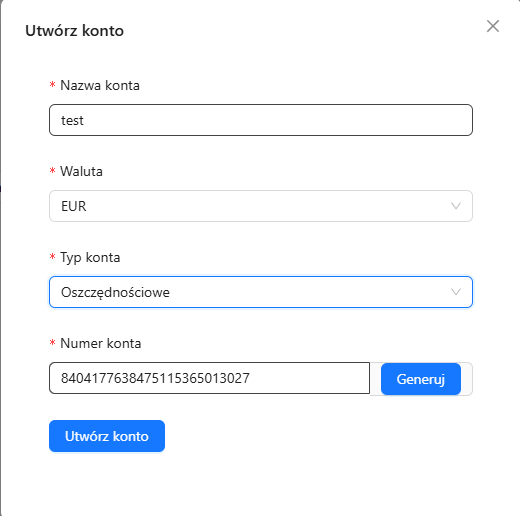
\includegraphics[width=0.7\linewidth]{images/AccountForm}
	\caption{Formularz dodania konta bankowego}
	\label{fig:accountform}
\end{figure}
Po utworzeniu konta możemy wejść w szczegóły naszego konta, gdzie zobaczymy wykresy z transakcjami, wszystkie transakcje i będziemy mogli posortować je dziennie lub wyświetlić wszystkie  (Rys. \ref{fig:accountpage}). Będziemy mieć również opcję wpłacenia gotówki na konto.
\begin{figure}
	\centering
	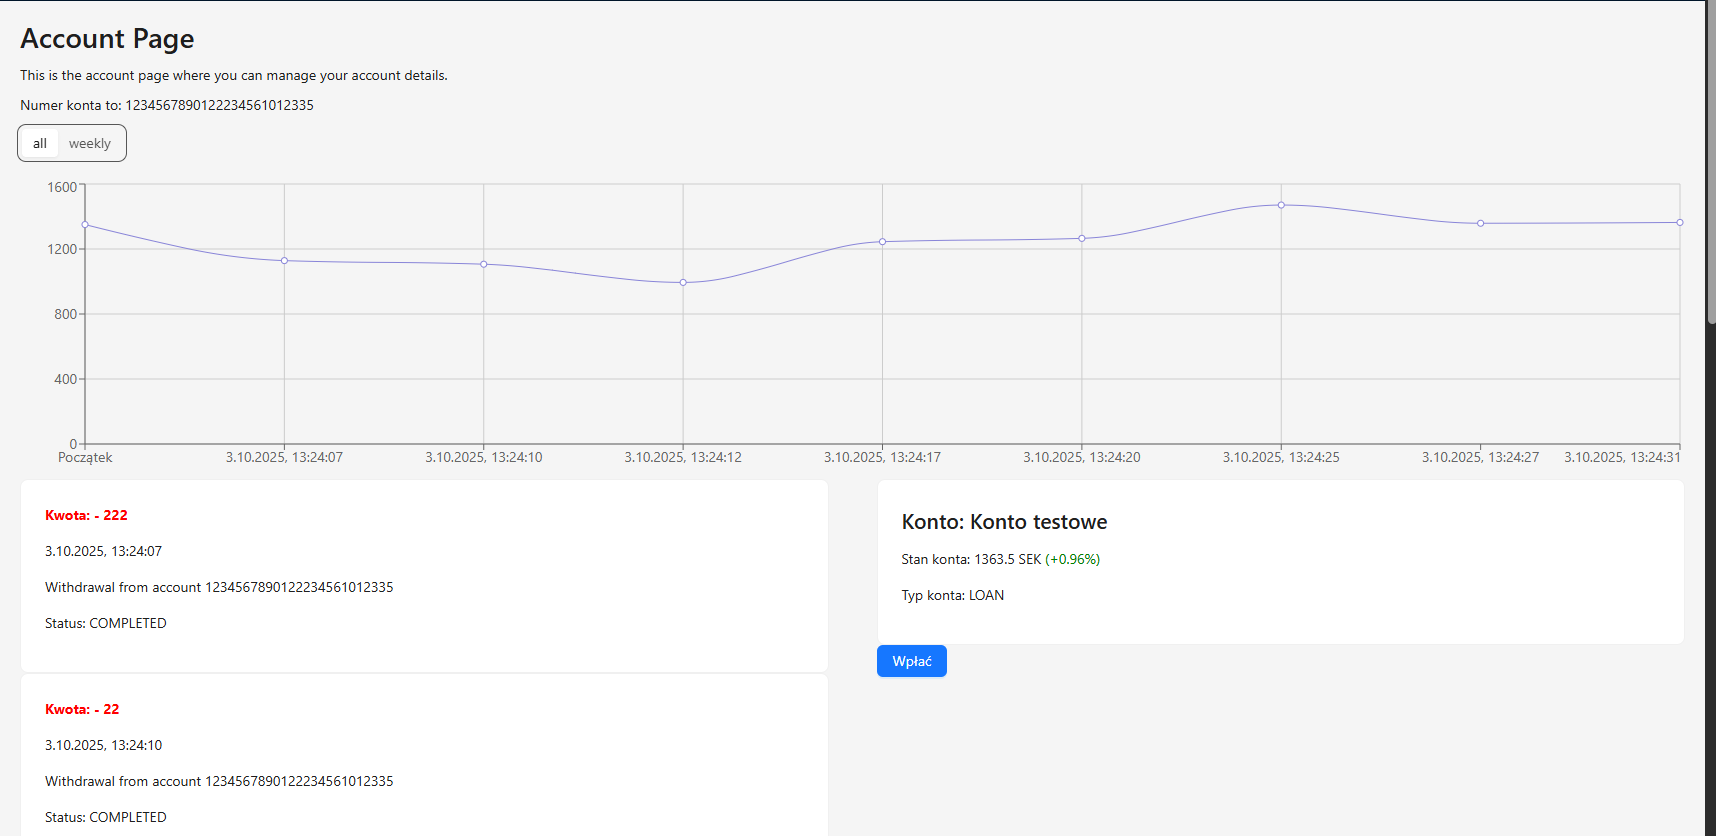
\includegraphics[width=0.7\linewidth]{images/AccountPage}
	\caption{Informacje o koncie użytkownika}
	\label{fig:accountpage}
\end{figure}
